\section{问题四：真实世界杯赛程的双层同口径评价}

\subsection{比较边界与数据来源}

本问选取 $2022$ 年卡塔尔世界杯小组赛作为现实参照。机器读取源为工作区保存的 OpenFootball 结构化 JSON，FIFA 官方赛程与比分页面用于逐场核验；场馆容量取 FIFA 赛后统计，坐标按 FIFA 场馆地址核对\upcite{openfootball_2022,fifa_qatar_schedule,fifa_qatar_at_glance}。实际赛程的 $48$ 场记录逐行保存球队、轮次、场馆、当地开球时间、UTC 时间和机器来源链接，不再把“采集源”与“官方核验源”写成同一字段。附件中的空白模板仅规定提交字段，不被当作观测数据；UTC 时间根据当地时间和 IANA 时区重新计算。

实际赛程与问题二的 $72$ 场方案在球队规模、比赛数量和场馆集合上并不相同，直接比较总收益会把规模效应误当作安排优劣。为此，我们设置双层评价：第一层由两套赛程共同调用一个结构函数，比较休息、跨时区、实际场馆旅行、场馆日负荷、容量匹配、黄金覆盖和预计观众；第二层先将现实比赛与场馆整体映射到问题二候选域，再复算问题二八指标。

流程的关键不是寻找一个绝对“冠军方案”，而是保持比较口径对称。结构层的每一项均有明确物理单位和规模分母；代理层的现实比赛与场馆分别整体映射到问题二的比赛和安保合格候选场馆，随后使用问题二相同的距离、时间、时区边界与权重。现实数据无法直接识别的商业、安保和题内吸引力统一标记为代理量，并与可观测结构分开解释。

\subsection{结构层的共同计算函数}

设球队 $t$ 的相邻两场比赛为 $j-1,j$，UTC 开球时刻为 $u_{tj}$，场馆坐标为 $(\phi_{tj},\lambda_{tj})$，场馆 UTC 偏移为 $z_{tj}$。休息、场馆旅行和跨时区指示分别定义为
\begin{equation}
r_{tj}=u_{tj}-u_{t,j-1},\qquad
d_{tj}=\operatorname{Haversine}\!\left((\phi_{t,j-1},\lambda_{t,j-1}),(\phi_{tj},\lambda_{tj})\right),
\end{equation}
\begin{equation}
c_{tj}=\mathbb I\!\left(z_{tj}\ne z_{t,j-1}\right).
\end{equation}
休息报告全部球队相邻轮间隔的最小值和平均值；旅行距离、换馆率和跨时区率均以球队转场次数为分母。场馆日利用率以“发生比赛的场馆日数”除以“启用场馆数乘比赛日期数”，场馆日峰值取单一场馆单日最大比赛数。容量匹配率为逐场 $\min(N_i/K_i,1)$ 的均值，黄金覆盖率和场均预计观众均以比赛场次为分母。两套赛程只传入字段名不同，计算公式和聚合方式完全相同。

\begin{table}[H]
\centering
\caption{两套赛程的可观测结构与规模强度比较}
\label{tab:q4-structural-comparison}
\small
\resizebox{\textwidth}{!}{%
\begin{tabular}{lllrrl}
\toprule
指标 & 定义与分母 & 单位 & 2022实际 & 2026优化 & 偏好方向 \\
\midrule
最小休息 & 球队相邻比赛 UTC 间隔的最小值 & 小时 & 87.0000 & 63.0000 & 越高越优 \\
平均休息 & 球队相邻比赛 UTC 间隔的平均值 & 小时 & 97.8125 & 139.8125 & 越高越优 \\
跨时区次数 & 相邻比赛场馆 UTC 偏移发生变化的次数 & 次 & 0 & 78 & 越低越优 \\
跨时区率 & 跨时区次数除以球队转场次数 & 比例 & 0.0000 & 81.2500 & 越低越优 \\
场馆旅行 & 相邻比赛实际场馆大圆距离的平均值 & 公里/次 & 18.9868 & 2019.1075 & 越低越优 \\
换馆率 & 相邻轮更换场馆的球队转场比例 & 比例 & 78.1250 & 94.7917 & 越低越优 \\
场馆日利用率 & 发生比赛的场馆日占可用场馆日比例 & 比例 & 45.1923 & 25.0000 & 越高越优 \\
场馆日峰值 & 单一场馆单日承办场次最大值 & 场/场馆日 & 2 & 1 & 越低越优 \\
容量匹配 & 预计现场观众与场馆容量之比的场均值 & 比例 & 81.7689 & 61.7245 & 越高越优 \\
黄金覆盖 & 按赛事进度日和 UTC 钟点映射后落入前四分位时段的比例 & 比例 & 25.0000 & 62.5000 & 越高越优 \\
场均预计观众 & 预计现场观众总量除以比赛场次 & 人/场 & 41451.67 & 41704.92 & 越高越优 \\
\bottomrule
\end{tabular}
}
\vspace{2pt}
\noindent\begin{minipage}{0.96\textwidth}\footnotesize 注：休息、时区、场馆路径与场馆日由逐场赛程直接复算；黄金覆盖来自唯一时段映射，容量匹配和预计观众的需求端为题内赛前代理。实际赛程有64次球队转场，优化赛程有96次。\end{minipage}
\end{table}


结构层逐项比较见表\ref{tab:q4-structural-comparison}。实际赛程最小休息为 $87$ 小时，高于优化方案的 $63$ 小时；但优化方案平均休息达到 $139.8125$ 小时，高于实际赛程的 $97.8125$ 小时，说明优化方案的休息分布更不均匀。卡塔尔赛程位于同一时区，$64$ 次球队转场中没有跨时区；跨国优化赛程的 $96$ 次转场中有 $78$ 次跨时区，平均场馆旅行距离也由 $18.9868$ 公里升至 $2019.1075$ 公里。

场馆运营维度呈现另一组取舍。实际与优化方案的场馆日峰值分别为 $2$ 场和 $1$ 场；场馆日利用率分别为 $45.1923\%$ 和 $25.0000\%$。基于同一赛前需求代理，两者的平均容量匹配率分别为 $81.7689\%$ 和 $61.7245\%$，场均预计现场观众分别为 $41451.67$ 和 $41704.92$ 人。按后述唯一时段映射，优化方案的黄金时段覆盖率为 $62.5000\%$，高于实际赛程的 $25.0000\%$；该项属于时间映射指标，不能替代跨时区和长距离旅行负担。

为统一展示不同物理单位下的方向和相对幅度，图\ref{fig:q4-schedule-difference}先按两方案绝对值最大者归一每个结构指标，再把“优化更符合偏好”记为正值。原始小时、公里、场次与比例仍以表\ref{tab:q4-structural-comparison}为准。

\begin{figure}[htbp]
    \centering
    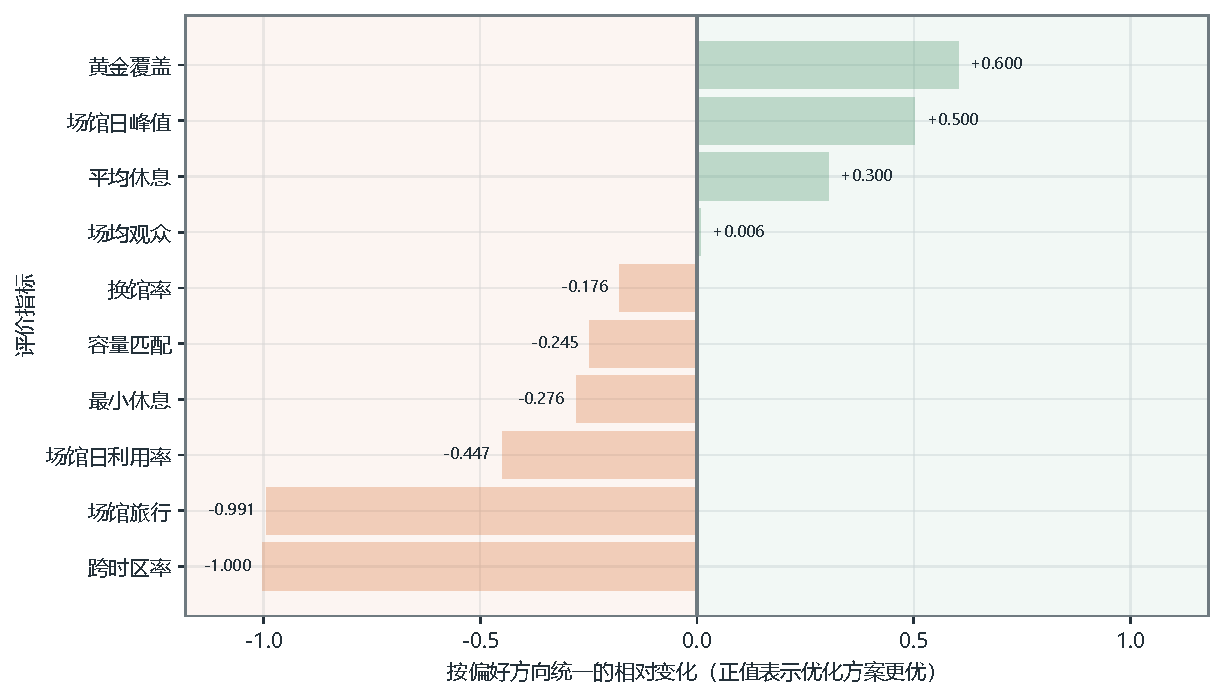
\includegraphics[width=0.85\textwidth,height=0.80\textheight,keepaspectratio]{../figures/fig_q4_schedule_difference.pdf}
    \caption{两套赛程的结构指标相对差异}
    \label{fig:q4-schedule-difference}
\end{figure}

\subsection{代理层的同构映射与强度化}

对受比赛数量影响的总量先做场均强度化。若方案 $s$ 有 $n_s$ 场比赛，则电视价值、品牌价值和成本分别写为
\begin{equation}
\bar T_s=\frac{T_s^0}{n_s},\qquad
\bar B_s=\frac{B_s^0}{n_s},\qquad
\bar C_s=\frac{C_s^0}{n_s}.
\end{equation}
旅行与风险使用逐场均值，$U,H$ 本身已是均值，公平性 $F$ 是每队三场资源次数极差的标准化结果。对 $T,B,C$，先将问题二候选上下界除以 $72$ 转为场均边界，再与基准实际、优化及第二近邻三个已报告场景的原始值取共同包络。两个方案随后共享这一组边界执行一次 Min--Max，既保留共同参照，又保证进入 $Z_4$ 的八项值严格属于 $[0,1]$。

实际赛程缺少与题目附件完全同构的商业和安保字段。为避免目标型特征和静默缺失填补，本文引入 $2022$ 年 $11$ 月 $12$ 日完整的世界杯赛前 Elo 快照\upcite{international_football_elo_2022}，覆盖全部 $32$ 支球队。比赛距离只使用双方 Elo 均值与差、由 Elo 构造的胜平负概率、不确定性和组内轮次，在题内 $72$ 场中寻找最近邻，再整体继承基础需求、吸引力与安保向量；预测观看人数不再参与邻居距离。实际场馆只依据有官方来源的容量，在满足该场安保等级的题内场馆中映射成本参数，不再声称使用逐场馆气候或公共交通数据。风险中的气候项固定为透明情景值 $0.12$。$U$ 不继承邻居，而由同一组三向赛前概率直接计算：
\begin{equation}
U_i=1-\max\{p_{ia},p_{iD},p_{ib}\}.
\end{equation}
黄金时段也复用问题二规则：先固定附件 $80$ 个候选时段中得分最高的 $20$ 个。为消除不同日期具有相同时钟距离时由行顺序决定结果的问题，先把现实赛程的 $13$ 个比赛日按赛事进度线性映射到模拟赛程的 $20$ 个候选日，再在对应日期内选择圆周 UTC 钟点距离最近的时段；若距离仍相同，则按时段编号稳定选择。由此每场现实比赛得到唯一、可复算的候选时段。

为保证两套赛程的旅行指标具有相同物理定义，现实赛程的每场比赛和场馆先整体映射到问题二索引，再调用问题二同一个旅行负担表；不把卡塔尔实际路径公里数除以全球最大距离后直接与问题二复合量混列：
\begin{equation}
D_i=\frac{1}{2}\sum_{t\in\{a_i,b_i\}}
\left(0.5\widetilde d_{tiv}+0.3\widetilde h_{tiv}+0.2\widetilde z_{tiv}\right).
\end{equation}
其中三项边界、第二三轮上一轮安保合格场馆集合与问题二完全一致。真实场馆路径仍在结构层以公里报告，不再进入这一复合量。

综合目标仅作为给定映射体系下的条件性分数：
\begin{equation}
Z_4=0.25T'+0.25B'+0.15U+0.10H-
\left(0.08C'+0.07D'+0.06F+0.04R\right).
\end{equation}

\subsection{代理指标结果与稳健性边界}

同构映射后，实际赛程的代理指标为 $T'=0.413433$、$B'=0.633928$、$U=0.441275$、$H=0.649119$、$C'=0.534340$、$D'=0.213022$、$F=0.666667$、$R=0.455654$；优化方案对应为 $0.918281$、$0.797646$、$0.461436$、$0.639699$、$0.382445$、$0.201797$、$0.333333$ 和 $0.416678$。八项值均位于 $[0,1]$，不再存在边界外推后由单一指标主导综合分的问题；各指标证据等级及单位列于附录表\ref{tab:q4-metric-definition}。

条件性代理层的共同尺度轮廓见附录图\ref{fig:q4-metric-radar}：优化方案在 $T,B,U,C,D,F,R$ 上更符合目标方向，实际赛程仅在 $H$ 上略高。成本、旅行、公平和风险在作图时只反转偏好方向，不再按两方案最大值二次缩放。由于这些指标的证据等级不同，雷达轮廓只能说明题内映射下的取舍，不能替代结构层的小时和公里结果。

基准最近邻代理下，实际赛程的 $Z_4$ 为 $0.277058$，优化赛程为 $0.480778$。逐一将八个权重的绝对值乘以 $0.9$ 和 $1.1$ 后重新归一，共形成 $16$ 个扰动情景：实际分位于 $[0.267908,0.285763]$，优化分位于 $[0.469560,0.491449]$，方向保持率为 $100\%$。将实际比赛与场馆代理整体换成第二近邻后，实际方案的 $Z_4$ 为 $0.226072$，优化方向仍保持。

修复后的代理方向在已检验权重和邻居替换下稳定，但证据边界仍不能省略：$48$ 场现实比赛映射到 $26$ 个题内比赛，单一比赛最多复用 $6$ 次；场馆成本代理只覆盖 $4$ 个题内场馆，其中一个被复用 $33$ 次。因此可以报告“当前题内映射下优化方案条件性总分较高”，却不能据此断言 FIFA 现实排程总体较差。抽签规则、转播合同、场馆可用性、当地治理、球队迁移策略和商业谈判等现实约束并未被附件完整观察；若用于现实决策，仍须补充真实合同、场馆运营和安保成本数据后重新校准代理层。
